\documentclass{article}
\usepackage[utf8]{inputenc} %кодировка
\usepackage[T2A]{fontenc}
\usepackage[english,russian]{babel} %русификатор 
\usepackage{mathtools} %библиотека матеши
\usepackage[left=1cm,right=1cm,top=2cm,bottom=2cm,bindingoffset=0cm]{geometry} %изменение отступов на листе
\usepackage{amsmath}
\usepackage{graphicx} %библиотека для графики и картинок
\graphicspath{}
\DeclareGraphicsExtensions{.pdf,.png,.jpg}
\usepackage{subcaption}
\usepackage{pgfplots}
\usepackage{float}

\begin{document}
% НАЧАЛО ТИТУЛЬНОГО ЛИСТА
\begin{center}
    \Large
    Федеральное государственное автономное \\
    образовательное учреждение высшего образования \\ 
    «Научно-образовательная корпорация ИТМО»\\
    \vspace{0.5cm}
    \large
    Факультет программной инженерии и компьютерной техники \\
    Направление подготовки 09.03.04 Программная инженерия \\
    \vspace{1cm}
    \Large
    \textbf{Отчёт по лабораторной работе №1} \\
        По дисциплине «Компьютерные сети» ( семестр 6)\\
    \large
    \vspace{8cm}

    \begin{minipage}{.33\textwidth}
    \end{minipage}
    \hfill
    \begin{minipage}{.4\textwidth}
    
        \textbf{Студент}: \vspace{.1cm} \\
        \ Дениченко Александр P3312\\
        \textbf{Практик}:  \\
        \ Тропченко Андрей Александрович
    \end{minipage}
    \vfill
Санкт-Петербург\\ 2025 г.
\end{center}
\pagestyle{empty}
% КОНЕЦ ТИТУЛЬНОГО ЛИСТА 
\newpage
\pagestyle{plain}

\section*{Цель работы}
\begin{itemize}
    \item Изучение принципов построения и настройки моделей компьютерных
    сетей в среде NetEmul.
    \item В процессе выполнения лабораторной работы (ЛР) необходимо:
    построить три простейшие модели компьютерной сети;
    \item Выполнить настройку сети, заключающуюся в присвоении IP-адресов
    интерфейсам сети;
    \item Выполнить тестирование разработанных сетей путем проведения
    экспериментов по передаче данных на основе протокола UDP;
    \item Сохранить разработанные модели компьютерных сетей для демонстрации
    процессов передачи данных при защите лабораторной работы.
\end{itemize}

\section*{Вариант}

Номер группы: P3312
\\
ФИО: Дениченко (9) Александр (9) Олегович (8)

Ф=9; И=9; О=8; Н=12
\\ \\
Первая сеть начальный адрес: 212.21.21.18
\\
Вторая сеть начальный адрес: 212.30.21.27
\\
Третья сеть начальный адрес: 212.21.29.26



\section{Этап первый}
Были добавлены 2 компьютера и по одной сетевый карте каждому.
Сетевые карты настроены на первую сеть.
\\
Так же была перекличка ARP реквестами (чтобы определить MAC адреса устройств в сети, изначально отправляется ARP на широковещательный адрес). 
После чего произошёл обмен UDP-сообщением на транспорном уровне, так как МАС адреса уже известны.
В самих UDP можно увидеть пакет с адресом отправителя, получателя и их порты.
\begin{center}
    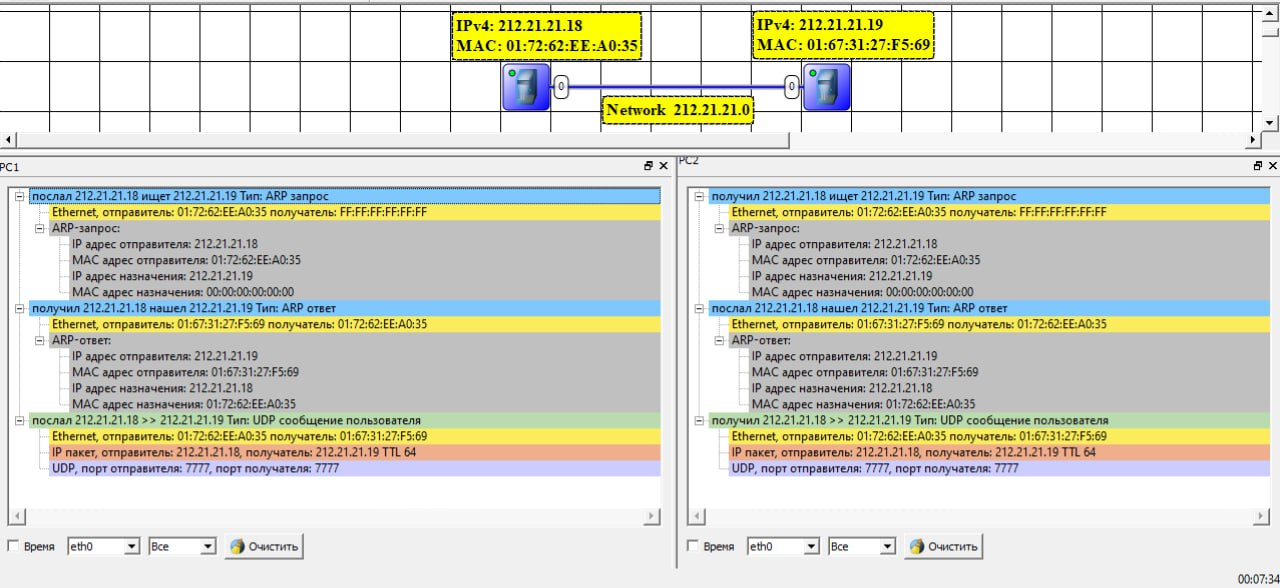
\includegraphics[width=.9\textwidth]{1}
\end{center}

В таблицах маршрутизации соответсвенно можно увидеть подключения сетевой карты: обозначено место назначения, маска, шлюз (через который пройдёт сообщение), интерфейс, метрика, тип источника.

\begin{center}
    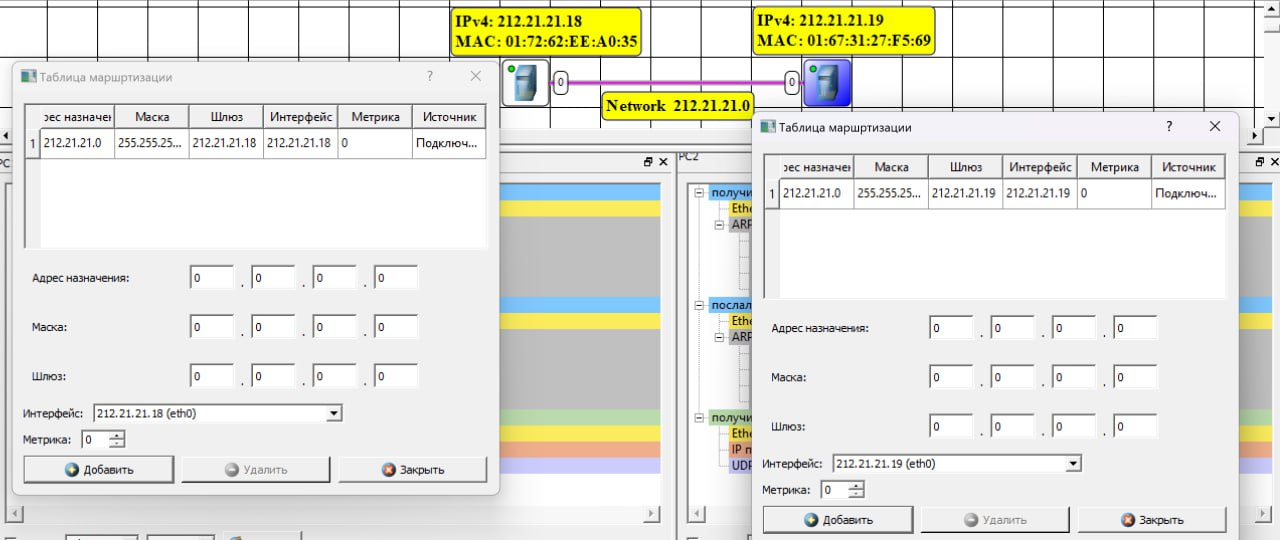
\includegraphics[width=.9\textwidth]{2}
\end{center}

В ARP таблице можно увидеть соответствие IP адреса к MAC в нашей сети.
\\
\begin{minipage}{.5\textwidth}    
    \begin{center}
        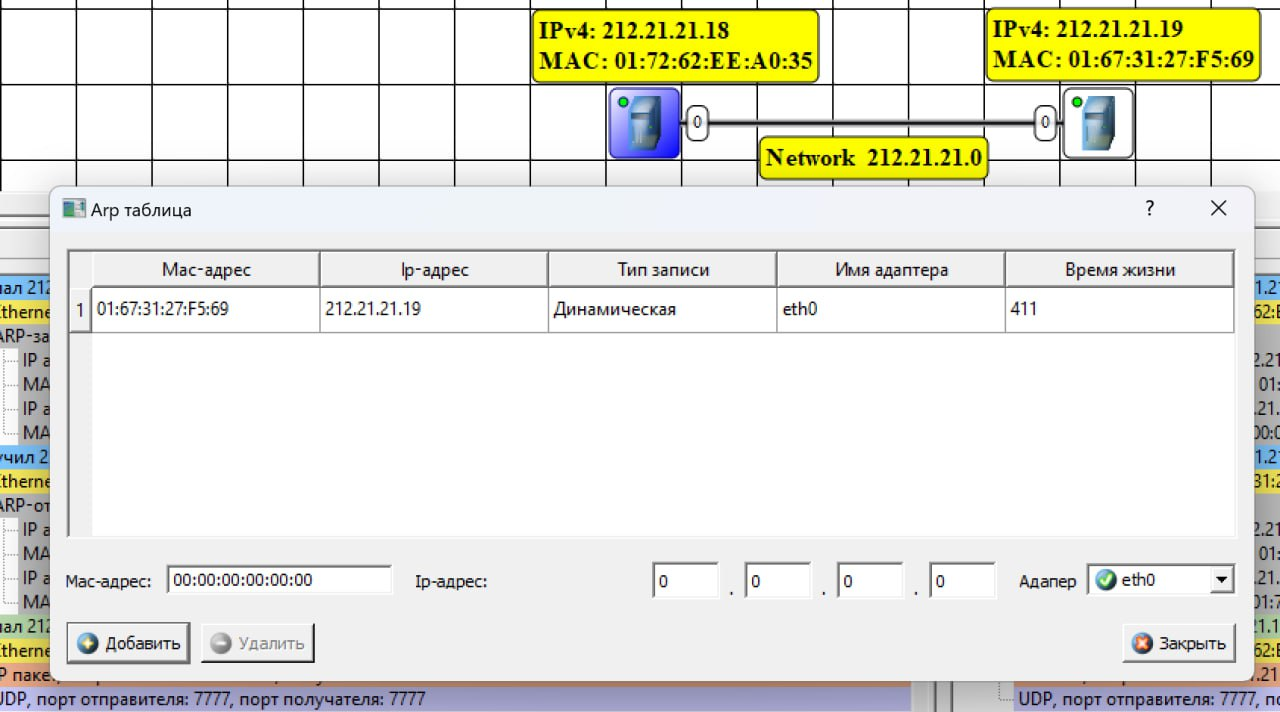
\includegraphics[width=.9\textwidth]{3}
    \end{center}
\end{minipage}
\hfil
\begin{minipage}{.5\textwidth}    
    \begin{center}
        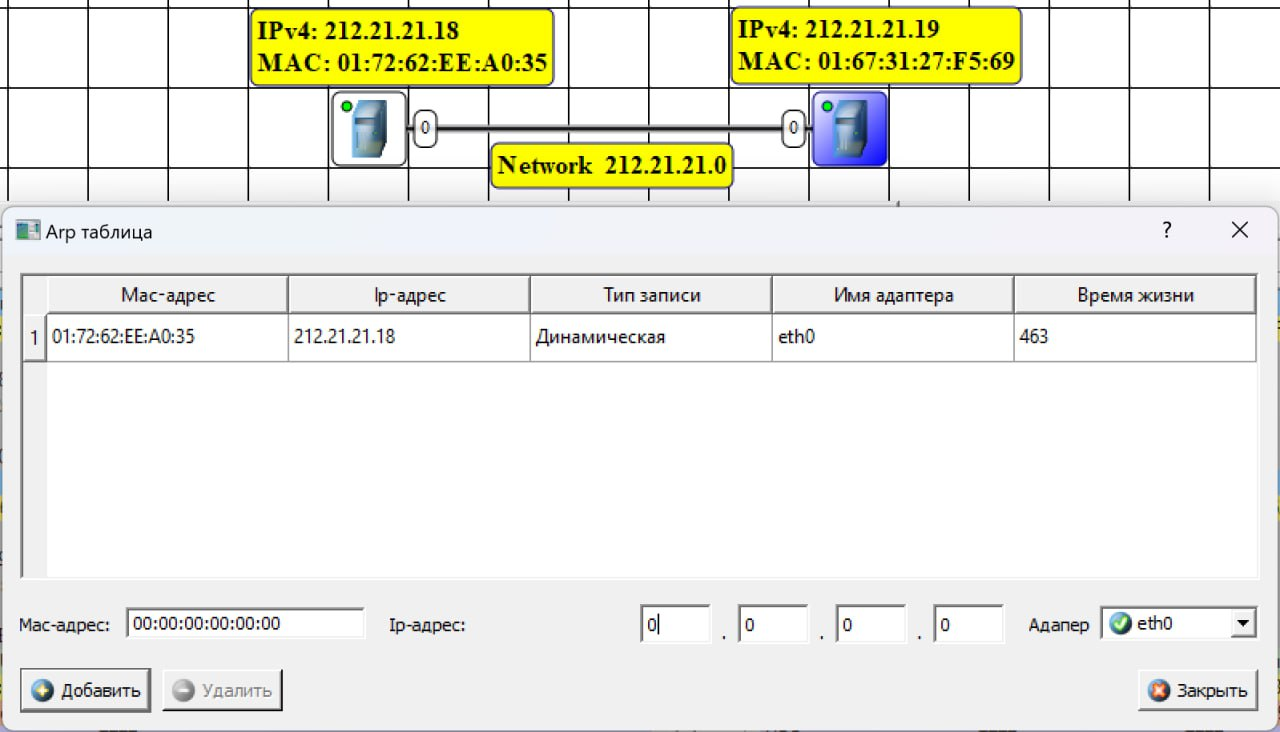
\includegraphics[width=.9\textwidth]{4}
    \end{center}
\end{minipage}
Тут содержатся следующие данные о подключении: физический адрес утройства, с которым произошло подключение; сетевой адрес этого устройства; тип записи (динамически, так как запись была добавлена автоматически); интерфейс, через который была получена информация; время жизни, в течении которого будет храниться запись в таблице, если не будет обновлена.

\section{Линейная компьютерная сеть}
\begin{center}
    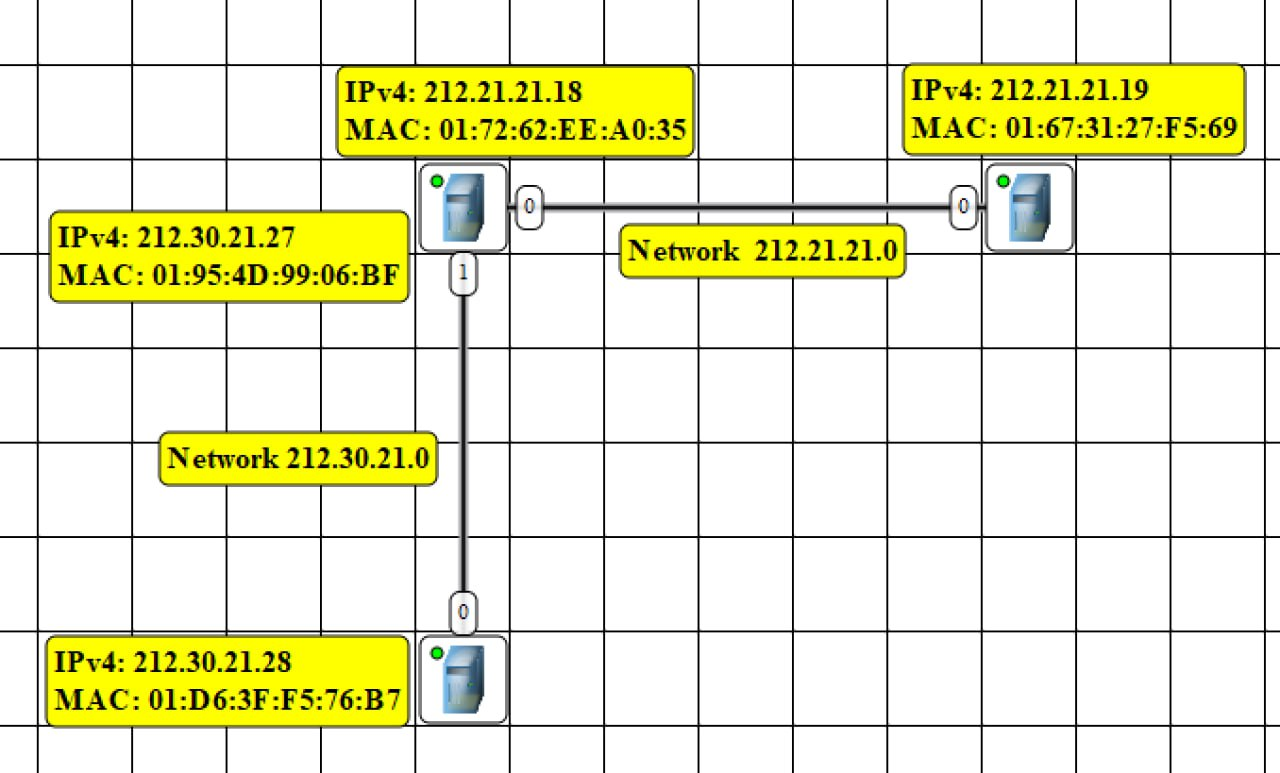
\includegraphics[width=.9\textwidth]{5}
\end{center}
Была добавлена ещё одна сеть и ПК3. У ПК1 включён раутинг и добавлена ещё один интерфейс для подключения к новой сети.

\begin{center}
    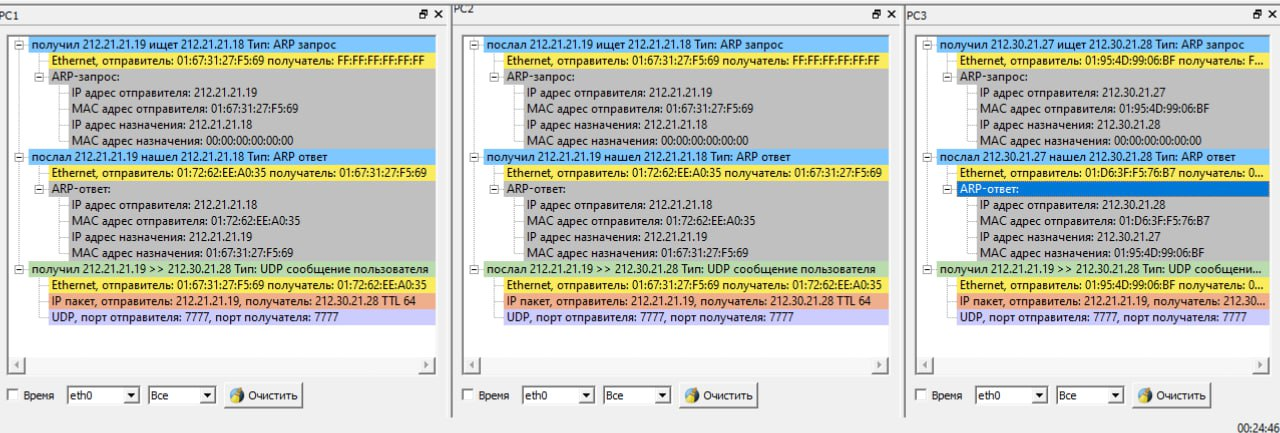
\includegraphics[width=.9\textwidth]{6}
\end{center}
Протестирована отправка пакета с крайнего ПК до другого крайнего. Изначально прошли ARP для определения устройств в каждой подсети.

\begin{center}
    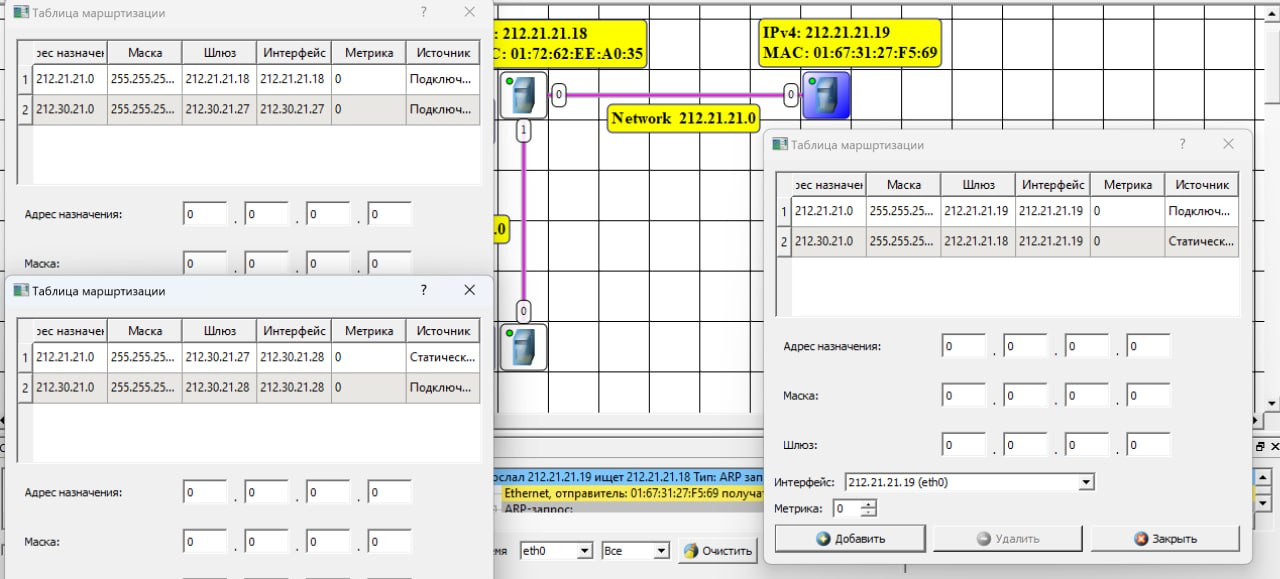
\includegraphics[width=.9\textwidth]{7}
\end{center}
В таблице маршрутизации у первого ПК появились записи, которые описывают подключения в обоих подсетях. 
Для корректной работы крайних компьютеров, определены статические пути, который показывают, как попасть в отличную нашей сеть. 

\begin{minipage}{.5\textwidth}    
    \begin{center}
        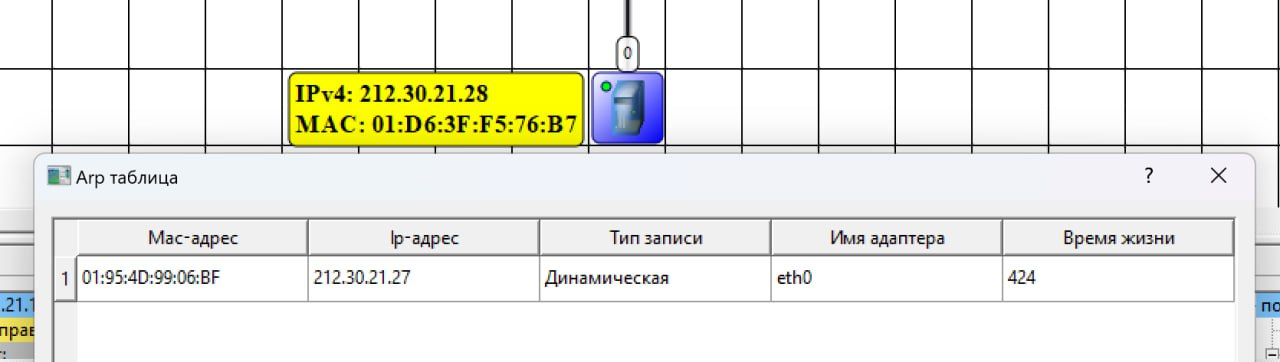
\includegraphics[width=.9\textwidth]{9}
    \end{center}
\end{minipage}
\hfill
\begin{minipage}{.5\textwidth}
    \begin{center}
        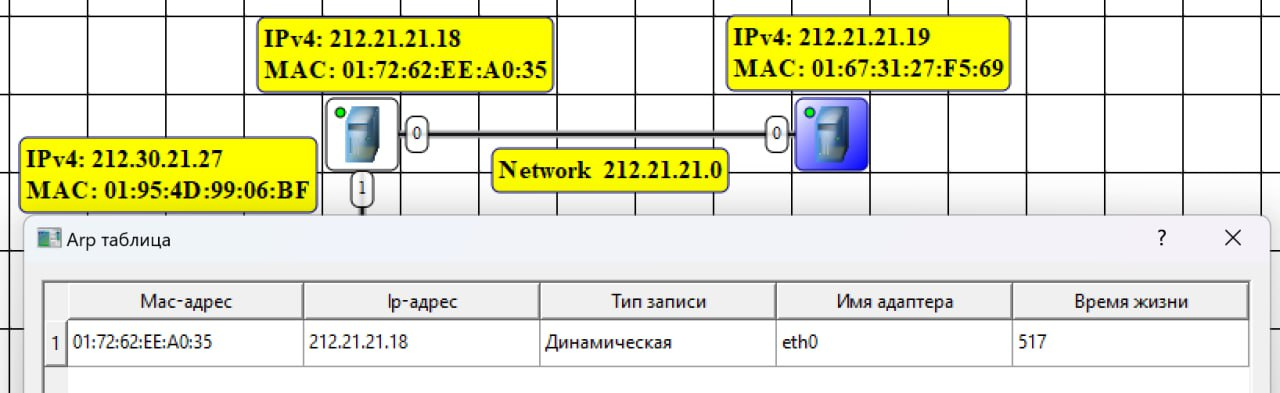
\includegraphics[width=.9\textwidth]{10}
    \end{center}
\end{minipage}
\begin{center}
    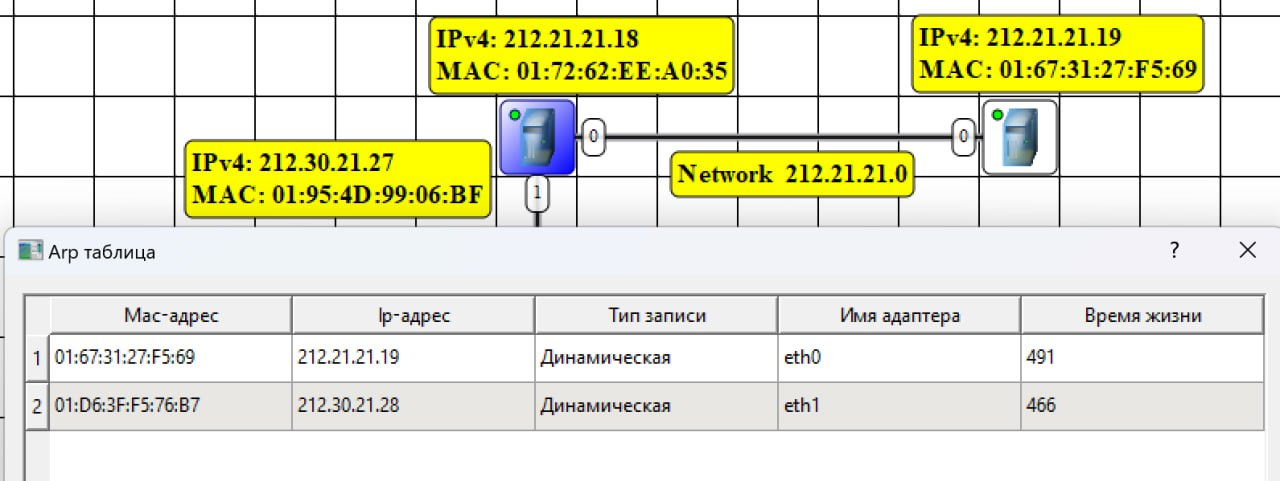
\includegraphics[width=.9\textwidth]{11}
\end{center}

\section{Полносвязная сеть}
Для построения полнослязной сети крайним ПК добавлены интерфейсы для добавления третьей подсети.
\begin{center}
    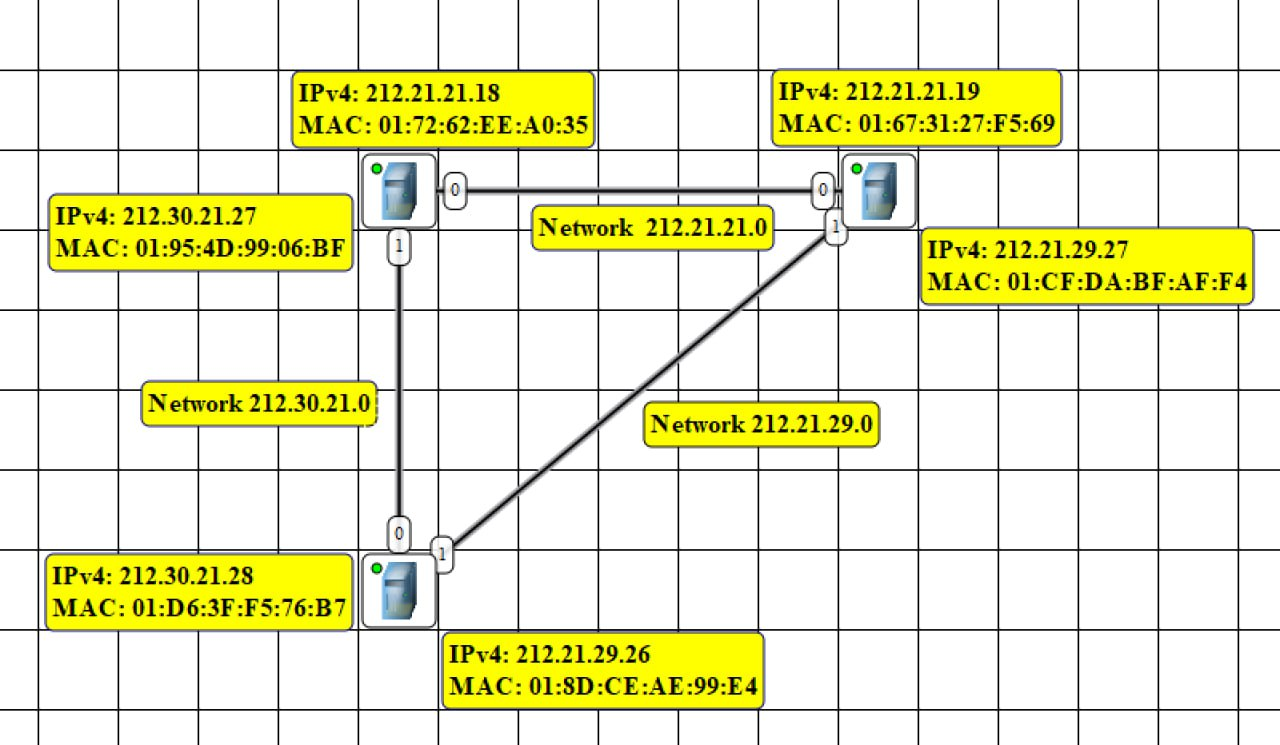
\includegraphics[width=.9\textwidth]{12}
\end{center}
Изменились таблицы маршрутизации, 
где более конкретно заданы пути для перехода из нашей сети, 
чтобы обеспечить отправку сообщения любым удобным способом.

\begin{center}
    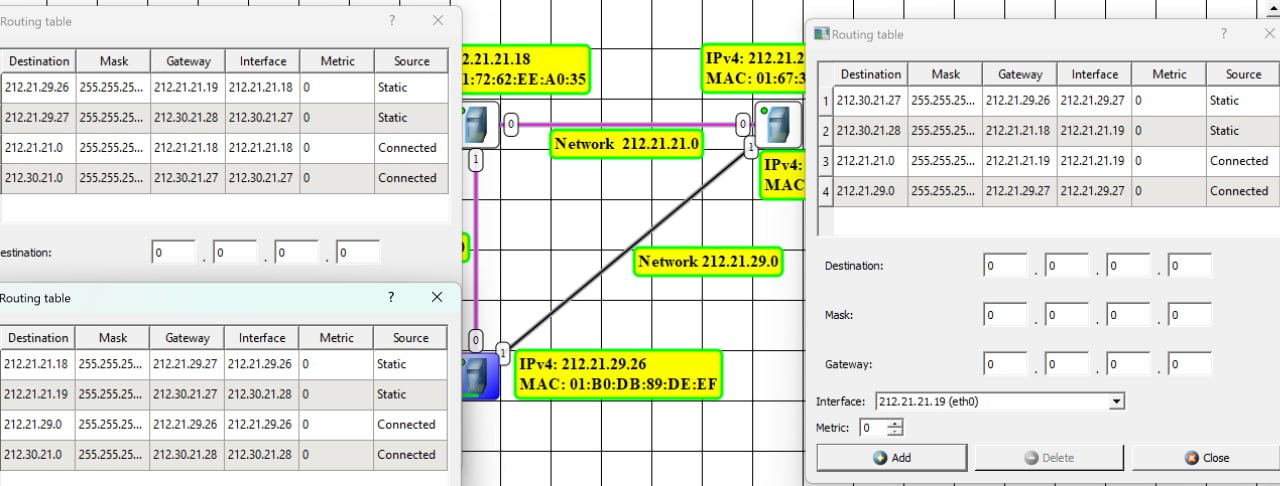
\includegraphics[width=.9\textwidth]{13}
\end{center}
Соответсвенно ARP таблицы тоже поменялись.

\begin{minipage}{.5\textwidth}
    \begin{center}
        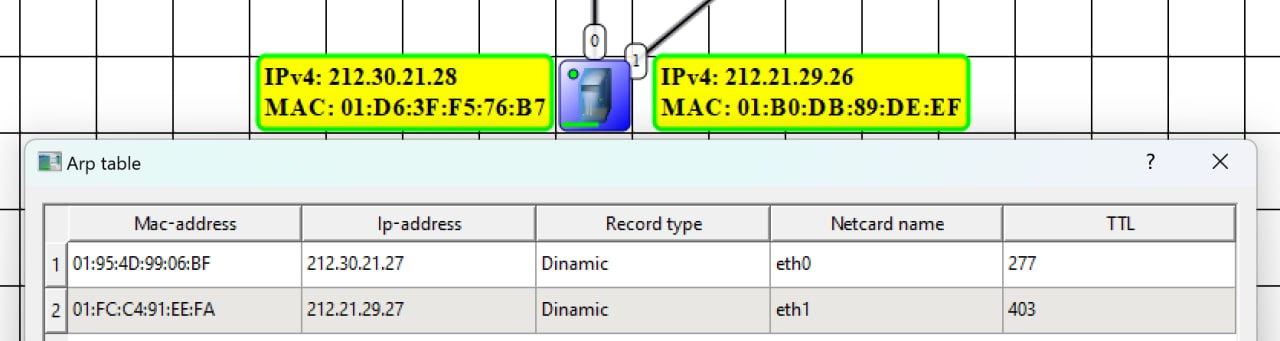
\includegraphics[width=.9\textwidth]{14}
    \end{center}
\end{minipage}
\hfill
\begin{minipage}{.5\textwidth}
    \begin{center}
        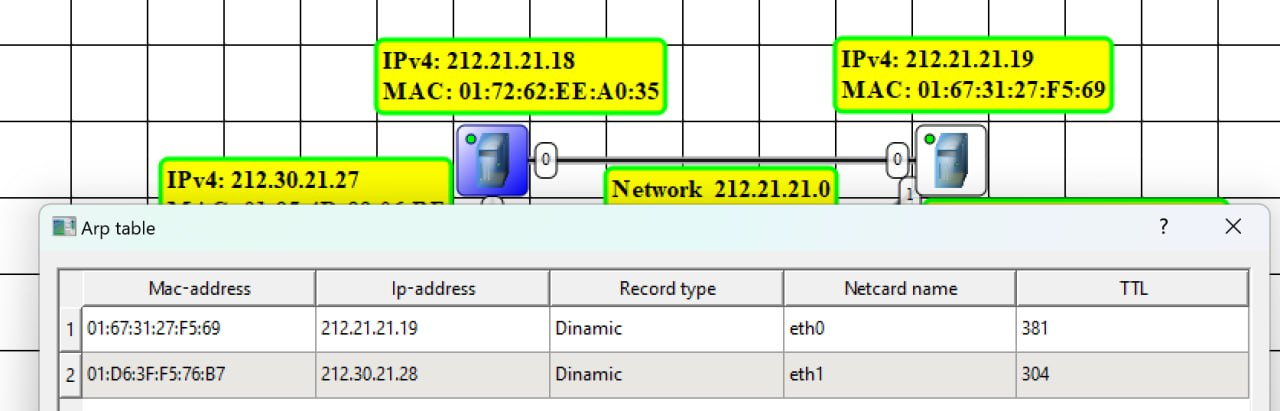
\includegraphics[width=.9\textwidth]{15}
    \end{center}
\end{minipage}

\begin{center}
    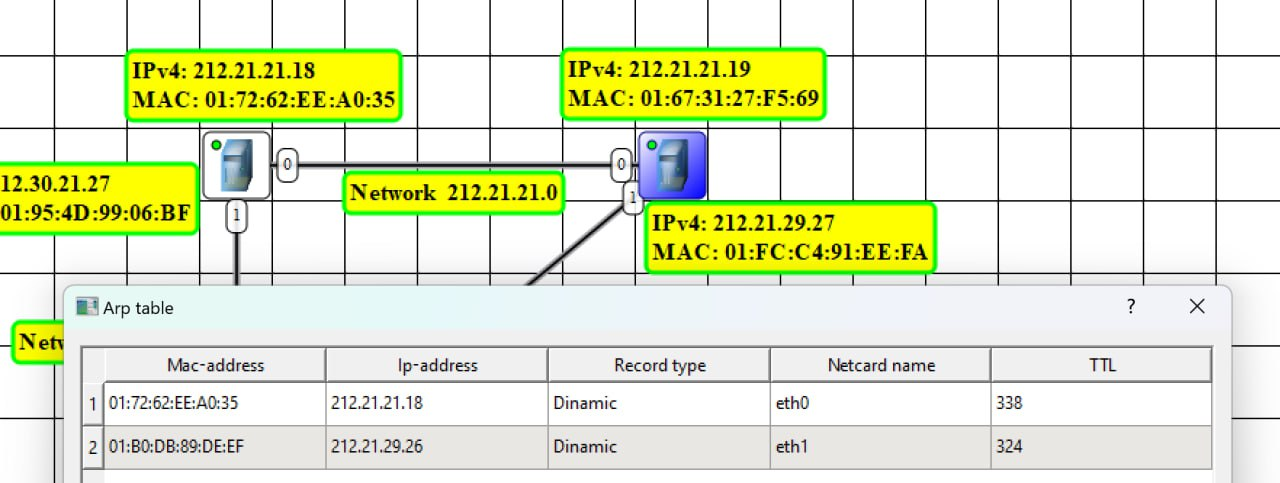
\includegraphics[width=.9\textwidth]{16}
\end{center}

\section*{Вывод}

В ходе лабораторной работы было:
\begin{itemize}
    \item Изучили принципы построения и настройки моделей компьютерных
    сетей в среде NetEmul.
    \item Построили три простейшие модели компьютерной сети;
    \item Выполнили настройку сети, заключающуюся в присвоении IP-адресов
    интерфейсам сети;
    \item Выполнили тестирование разработанных сетей путем проведения
    экспериментов по передаче данных на основе протокола UDP;
\end{itemize}

\end{document}
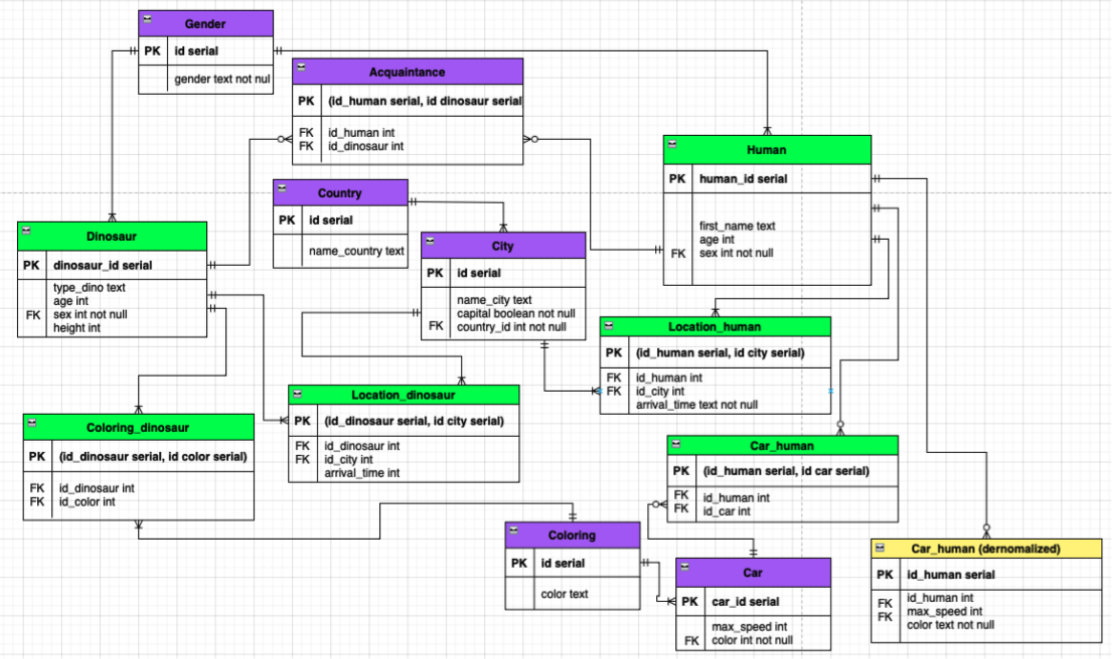
\includegraphics[width=.9\textwidth]{123}